\documentclass{standalone}
\usepackage{tikz}
\usetikzlibrary{patterns, positioning}
\usetikzlibrary{shapes.misc}
\usepackage[outline]{contour}
\contourlength{1.5pt} 
\usepackage[sfdefault]{ClearSans} %% option 'sfdefault' activates Clear Sans as the default text font
\usepackage[T1]{fontenc}

\begin{document}
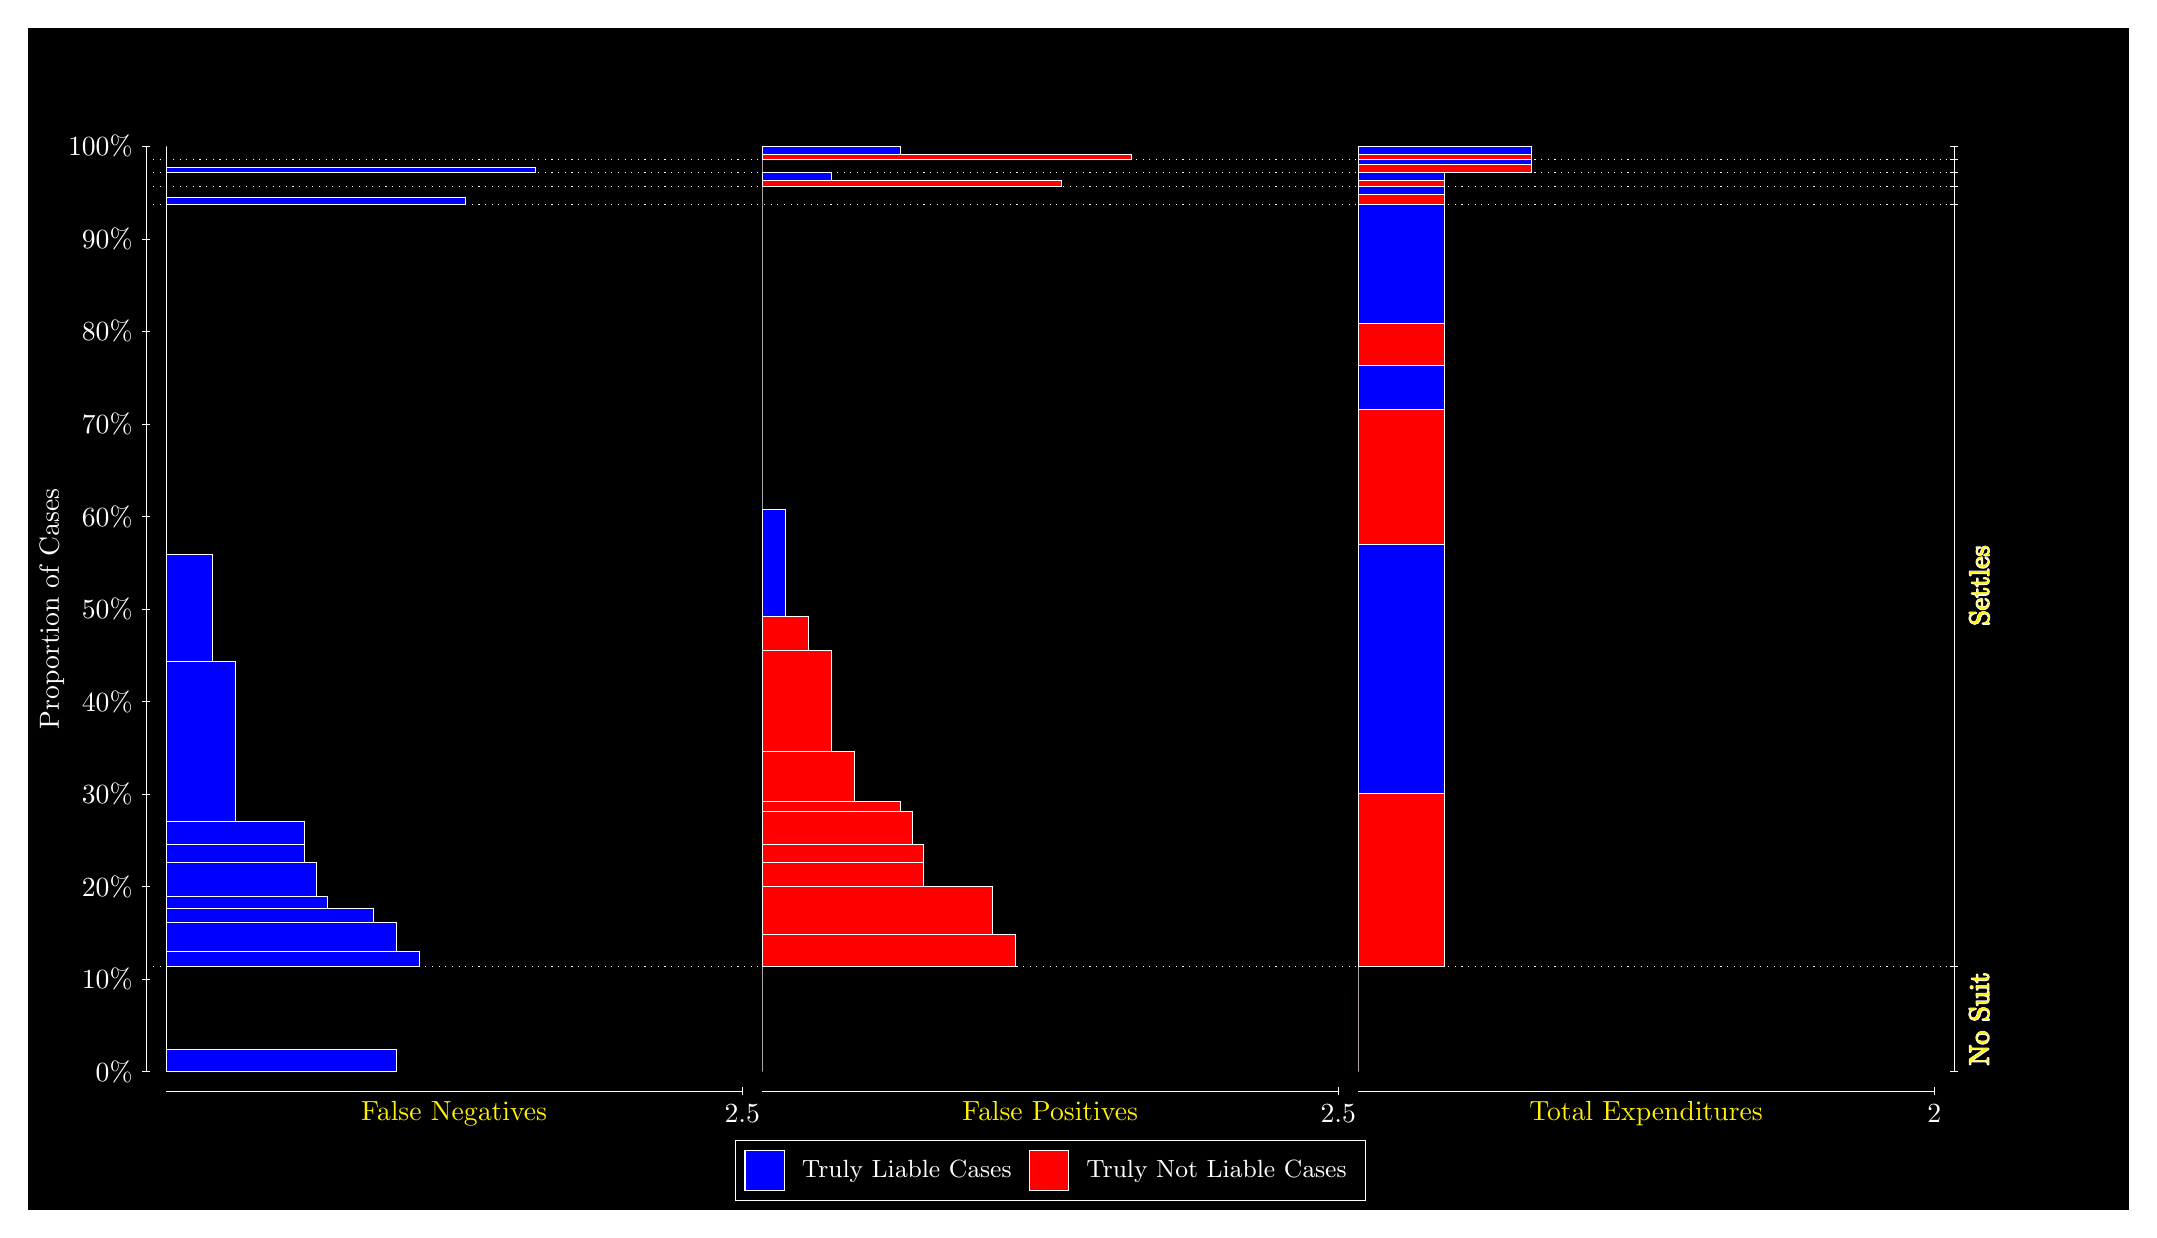
\begin{tikzpicture}
\draw[fill=black] (0,0) rectangle (26.667,15);
\draw[white, very thin] (1.5,1.75) -- (1.5,13.5);
\node[rotate=90, text=white, anchor=center] at (0.3, 7.625) {Proportion of Cases};
\draw[white, very thin] (1.45,1.75) -- (1.55,1.75);
\node[text=white, anchor=east] at (1.45, 1.75) {0\%};
\draw[white, very thin] (1.45,2.925) -- (1.55,2.925);
\node[text=white, anchor=east] at (1.45, 2.925) {10\%};
\draw[white, very thin] (1.45,4.1) -- (1.55,4.1);
\node[text=white, anchor=east] at (1.45, 4.1) {20\%};
\draw[white, very thin] (1.45,5.275) -- (1.55,5.275);
\node[text=white, anchor=east] at (1.45, 5.275) {30\%};
\draw[white, very thin] (1.45,6.45) -- (1.55,6.45);
\node[text=white, anchor=east] at (1.45, 6.45) {40\%};
\draw[white, very thin] (1.45,7.625) -- (1.55,7.625);
\node[text=white, anchor=east] at (1.45, 7.625) {50\%};
\draw[white, very thin] (1.45,8.8) -- (1.55,8.8);
\node[text=white, anchor=east] at (1.45, 8.8) {60\%};
\draw[white, very thin] (1.45,9.975) -- (1.55,9.975);
\node[text=white, anchor=east] at (1.45, 9.975) {70\%};
\draw[white, very thin] (1.45,11.15) -- (1.55,11.15);
\node[text=white, anchor=east] at (1.45, 11.15) {80\%};
\draw[white, very thin] (1.45,12.325) -- (1.55,12.325);
\node[text=white, anchor=east] at (1.45, 12.325) {90\%};
\draw[white, very thin] (1.45,13.5) -- (1.55,13.5);
\node[text=white, anchor=east] at (1.45, 13.5) {100\%};

\draw[white, very thin] (24.457,1.75) -- (24.457,13.5);
\draw[white, very thin] (24.407,1.75) -- (24.507,1.75);
\node[anchor=west] at (24.407, 1.75) {};
\draw[white, very thin] (24.407,3.0863) -- (24.507,3.0863);
\node[anchor=west] at (24.407, 3.0863) {};
\draw[white, very thin] (24.407,12.758) -- (24.507,12.758);
\node[anchor=west] at (24.407, 12.758) {};
\draw[white, very thin] (24.407,12.993) -- (24.507,12.993);
\node[anchor=west] at (24.407, 12.993) {};
\draw[white, very thin] (24.407,13.168) -- (24.507,13.168);
\node[anchor=west] at (24.407, 13.168) {};
\draw[white, very thin] (24.407,13.335) -- (24.507,13.335);
\node[anchor=west] at (24.407, 13.335) {};
\draw[white, very thin] (24.407,13.5) -- (24.507,13.5);
\node[anchor=west] at (24.407, 13.5) {};

\draw[white, very thin, fill=blue] (1.75,1.75) rectangle (4.6775,2.0365);
\draw[white, very thin, fill=red] (1.75,2.0365) rectangle (1.75,3.0863);
\draw[white, very thin, fill=blue] (1.75,3.0863) rectangle (4.9703,3.2741);
\draw[white, very thin, fill=blue] (1.75,3.2741) rectangle (4.6775,3.6409);
\draw[white, very thin, fill=blue] (1.75,3.6409) rectangle (4.3848,3.8249);
\draw[white, very thin, fill=blue] (1.75,3.8249) rectangle (3.7993,3.9747);
\draw[white, very thin, fill=blue] (1.75,3.9747) rectangle (3.6529,4.4035);
\draw[white, very thin, fill=blue] (1.75,4.4035) rectangle (3.5065,4.6314);
\draw[white, very thin, fill=blue] (1.75,4.6314) rectangle (3.5065,4.9324);
\draw[white, very thin, fill=blue] (1.75,4.9324) rectangle (2.6283,6.9571);
\draw[white, very thin, fill=blue] (1.75,6.9571) rectangle (2.3355,8.3127);
\draw[white, very thin, fill=red] (1.75,8.3127) rectangle (1.75,12.758);
\draw[white, very thin, fill=blue] (1.75,12.758) rectangle (5.5558,12.857);
\draw[white, very thin, fill=red] (1.75,12.857) rectangle (1.75,12.993);
\draw[white, very thin, fill=red] (1.75,12.993) rectangle (1.75,13.07);
\draw[white, very thin, fill=blue] (1.75,13.07) rectangle (1.75,13.168);
\draw[white, very thin, fill=blue] (1.75,13.168) rectangle (6.4341,13.235);
\draw[white, very thin, fill=red] (1.75,13.235) rectangle (1.75,13.335);
\draw[white, very thin, fill=red] (1.75,13.335) rectangle (1.75,13.401);
\draw[white, very thin, fill=blue] (1.75,13.401) rectangle (1.75,13.5);
\draw[white, very thin, fill=red] (9.3189,1.75) rectangle (9.3189,2.7997);
\draw[white, very thin, fill=blue] (9.3189,2.7997) rectangle (9.3189,3.0863);
\draw[white, very thin, fill=red] (9.3189,3.0863) rectangle (12.539,3.4947);
\draw[white, very thin, fill=red] (9.3189,3.4947) rectangle (12.246,4.1051);
\draw[white, very thin, fill=red] (9.3189,4.1051) rectangle (11.368,4.4061);
\draw[white, very thin, fill=red] (9.3189,4.4061) rectangle (11.368,4.6392);
\draw[white, very thin, fill=red] (9.3189,4.6392) rectangle (11.222,5.0503);
\draw[white, very thin, fill=red] (9.3189,5.0503) rectangle (11.075,5.1779);
\draw[white, very thin, fill=red] (9.3189,5.1779) rectangle (10.49,5.8197);
\draw[white, very thin, fill=red] (9.3189,5.8197) rectangle (10.197,7.1036);
\draw[white, very thin, fill=red] (9.3189,7.1036) rectangle (9.9044,7.5318);
\draw[white, very thin, fill=blue] (9.3189,7.5318) rectangle (9.6116,8.8875);
\draw[white, very thin, fill=blue] (9.3189,8.8875) rectangle (9.3189,12.758);
\draw[white, very thin, fill=red] (9.3189,12.758) rectangle (9.3189,12.895);
\draw[white, very thin, fill=blue] (9.3189,12.895) rectangle (9.3189,12.993);
\draw[white, very thin, fill=red] (9.3189,12.993) rectangle (13.125,13.07);
\draw[white, very thin, fill=blue] (9.3189,13.07) rectangle (10.197,13.168);
\draw[white, very thin, fill=red] (9.3189,13.168) rectangle (9.3189,13.268);
\draw[white, very thin, fill=blue] (9.3189,13.268) rectangle (9.3189,13.335);
\draw[white, very thin, fill=red] (9.3189,13.335) rectangle (14.003,13.401);
\draw[white, very thin, fill=blue] (9.3189,13.401) rectangle (11.075,13.5);
\draw[white, very thin, fill=red] (16.888,1.75) rectangle (16.888,2.7997);
\draw[white, very thin, fill=blue] (16.888,2.7997) rectangle (16.888,3.0863);
\draw[white, very thin, fill=red] (16.888,3.0863) rectangle (17.986,5.2837);
\draw[white, very thin, fill=blue] (16.888,5.2837) rectangle (17.986,8.4501);
\draw[white, very thin, fill=red] (16.888,8.4501) rectangle (17.986,10.162);
\draw[white, very thin, fill=blue] (16.888,10.162) rectangle (17.986,10.717);
\draw[white, very thin, fill=red] (16.888,10.717) rectangle (17.986,11.253);
\draw[white, very thin, fill=blue] (16.888,11.253) rectangle (17.986,12.758);
\draw[white, very thin, fill=red] (16.888,12.758) rectangle (17.986,12.895);
\draw[white, very thin, fill=blue] (16.888,12.895) rectangle (17.986,12.993);
\draw[white, very thin, fill=red] (16.888,12.993) rectangle (17.986,13.07);
\draw[white, very thin, fill=blue] (16.888,13.07) rectangle (17.986,13.168);
\draw[white, very thin, fill=red] (16.888,13.168) rectangle (19.083,13.268);
\draw[white, very thin, fill=blue] (16.888,13.268) rectangle (19.083,13.335);
\draw[white, very thin, fill=red] (16.888,13.335) rectangle (19.083,13.401);
\draw[white, very thin, fill=blue] (16.888,13.401) rectangle (19.083,13.5);
\draw[white, dotted] (1.5,3.0863) -- (24.457,3.0863);
\draw[white, dotted] (1.5,12.758) -- (24.457,12.758);
\draw[white, dotted] (1.5,12.993) -- (24.457,12.993);
\draw[white, dotted] (1.5,13.168) -- (24.457,13.168);
\draw[white, dotted] (1.5,13.335) -- (24.457,13.335);
\draw[white, very thin] (1.75,1.5) -- (9.0689,1.5);
\node[text=yellow, anchor=north] at (5.4094, 1.5) {False Negatives};
\draw[white, very thin] (9.0689,1.45) -- (9.0689,1.55);
\node[text=white, anchor=north] at (9.0689, 1.45) {2.5};

\draw[white, very thin] (9.3189,1.5) -- (16.638,1.5);
\node[text=yellow, anchor=north] at (12.978, 1.5) {False Positives};
\draw[white, very thin] (16.638,1.45) -- (16.638,1.55);
\node[text=white, anchor=north] at (16.638, 1.45) {2.5};

\draw[white, very thin] (16.888,1.5) -- (24.207,1.5);
\node[text=yellow, anchor=north] at (20.547, 1.5) {Total Expenditures};
\draw[white, very thin] (24.207,1.45) -- (24.207,1.55);
\node[text=white, anchor=north] at (24.207, 1.45) {2};

\node[text=yellow, centered, rotate=90] at (24.777, 2.4181) {\contour{white}{No Suit}};
\node[text=yellow, centered, rotate=90] at (24.777, 7.9223) {\contour{white}{Settles}};





\draw (12.978300999999998,1.5) node[draw=none] (baseCoordinate) {};
\begin{scope}[align=center]
        \matrix[scale=0.5, draw=white, below=0.5cm of baseCoordinate, nodes={draw}, column sep=0.1cm]{
            \node[rectangle, draw, minimum width=0.5cm, minimum height=0.5cm, fill=blue] {}; &
            \node[draw=none, font=\small, text=white] (B) {Truly Liable Cases}; &
            \node[rectangle, draw, minimum width=0.5cm, minimum height=0.5cm, fill=red] {}; &
            \node[draw=none, font=\small, text=white] (B) {Truly Not Liable Cases}; \\
            };
\end{scope}

\end{tikzpicture}
\end{document}